% 基礎数学 第11回 行列の基礎（CC BY-SA 4.0）
\documentclass[aspectratio=169]{beamer}
\usepackage{lfs-slides}
\lfscourse{基礎数学}

\title{行列の基礎}
\subtitle{基礎数学 第11回}
\author{}
\date{}

\begin{document}

\begin{frame}
  \titlepage
\end{frame}

\begin{frame}{今日のねらい}
  \lfsmessage{行列 ＝ 数を長方形に並べたもの。図形を動かす道具になる}
  \bigskip
  \begin{itemize}
    \item 行列の表し方（行・列・成分）
    \item 和・スカラー倍・積の計算
    \item 積の順番を入れ替えると結果が変わる
    \item 単位行列・零行列
    \item 工学では：コンピュータグラフィックスの回転
  \end{itemize}
\end{frame}

\section{行列とは}

\begin{frame}{行列の表し方}
  \begin{columns}[c]
    \column{0.5\textwidth}
      \[
        A = \begin{pmatrix} 1 & 2 & 3 \\ 4 & 5 & 6 \end{pmatrix}
      \]
      \begin{itemize}
        \item 横の並び：\textbf{行}（上から第1行、第2行）
        \item 縦の並び：\textbf{列}（左から第1列、第2列、第3列）
        \item 2行3列なので「$2 \times 3$ 行列」
      \end{itemize}
    \column{0.5\textwidth}
      \begin{block}{成分}
        第 $i$ 行・第 $j$ 列の数を $(i,\,j)$ 成分といい、$a_{ij}$ と書く
        \medskip

        例：$A$ の $(2,\,3)$ 成分は $a_{23} = 6$
      \end{block}
  \end{columns}
\end{frame}

\section{和・スカラー倍}

\begin{frame}{和とスカラー倍：同じ場所どうし}
  \lfsmessage{同じ大きさの行列なら、成分ごとに計算する}
  \[
    \begin{pmatrix} 1 & 2 \\ 3 & 4 \end{pmatrix}
    + \begin{pmatrix} 5 & 0 \\ -1 & 2 \end{pmatrix}
    = \begin{pmatrix} 6 & 2 \\ 2 & 6 \end{pmatrix}
  \]
  \[
    3 \begin{pmatrix} 1 & 2 \\ 3 & 4 \end{pmatrix}
    = \begin{pmatrix} 3 & 6 \\ 9 & 12 \end{pmatrix}
  \]
  {\small 大きさ（行の数・列の数）が違う行列は足せない}
\end{frame}

\section{積}

\begin{frame}{積：行と列をかけて足す}
  \lfsmessage{（左の行）×（右の列）}
  \[
    \begin{pmatrix} \alert{1} & \alert{2} \\ 3 & 4 \end{pmatrix}
    \begin{pmatrix} \alert{5} \\ \alert{6} \end{pmatrix}
    = \begin{pmatrix} \alert{1 \cdot 5 + 2 \cdot 6} \\ 3 \cdot 5 + 4 \cdot 6 \end{pmatrix}
    = \begin{pmatrix} 17 \\ 39 \end{pmatrix}
  \]
  \medskip
  \begin{block}{大きさの約束}
    $(m \times \alert{n})$ 行列 × $(\alert{n} \times p)$ 行列 ＝ $(m \times p)$ 行列\\
    {\small 左の列の数と右の行の数が同じときだけ計算できる}
  \end{block}
\end{frame}

\begin{frame}{$2 \times 2$ 行列どうしの積}
  \[
    \begin{pmatrix} 1 & 2 \\ 3 & 4 \end{pmatrix}
    \begin{pmatrix} 5 & 6 \\ 7 & 8 \end{pmatrix}
    = \begin{pmatrix}
        1 \cdot 5 + 2 \cdot 7 & 1 \cdot 6 + 2 \cdot 8 \\
        3 \cdot 5 + 4 \cdot 7 & 3 \cdot 6 + 4 \cdot 8
      \end{pmatrix}
    = \begin{pmatrix} 19 & 22 \\ 43 & 50 \end{pmatrix}
  \]
  \medskip
  {\small $(i,\,j)$ 成分 ＝ 左の第 $i$ 行 と 右の第 $j$ 列 をかけて足したもの}
\end{frame}

\begin{frame}{順番を入れ替えると？}
  $A = \begin{pmatrix} 1 & 2 \\ 3 & 4 \end{pmatrix}$，\
  $B = \begin{pmatrix} 5 & 6 \\ 7 & 8 \end{pmatrix}$ のとき
  \[
    AB = \begin{pmatrix} 19 & 22 \\ 43 & 50 \end{pmatrix}, \qquad
    BA = \begin{pmatrix} 23 & 34 \\ 31 & 46 \end{pmatrix}
  \]
  \lfsmessage{$AB \neq BA$：かける順番が大事}
\end{frame}

\begin{frame}{単位行列と零行列}
  \begin{columns}[t]
    \column{0.5\textwidth}
      \begin{block}{単位行列 $E$}
        \[
          E = \begin{pmatrix} 1 & 0 \\ 0 & 1 \end{pmatrix}
        \]
        $AE = EA = A$\\
        {\small 数の「$1$」の役割}
      \end{block}
    \column{0.5\textwidth}
      \begin{block}{零行列 $O$}
        \[
          O = \begin{pmatrix} 0 & 0 \\ 0 & 0 \end{pmatrix}
        \]
        $A + O = A$，\ $AO = OA = O$\\
        {\small 数の「$0$」の役割}
      \end{block}
  \end{columns}
\end{frame}

\section{工学では}

\begin{frame}{コンピュータグラフィックスの回転}
  \begin{columns}[c]
    \column{0.48\textwidth}
      \begin{center}
        % 原点のまわりの 90° 回転：P(2, 1) → P'(-1, 2)。三角形 OPQ ごと回す
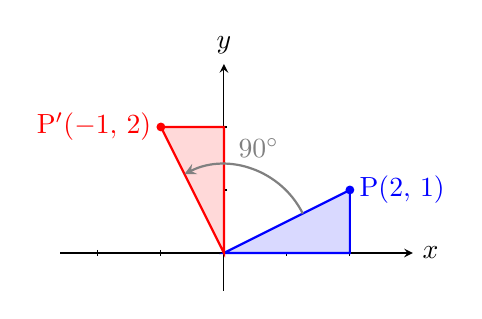
\begin{tikzpicture}[scale=0.8,>=stealth]
  \draw[->] (-2.6,0) -- (3,0) node[right] {$x$};
  \draw[->] (0,-0.6) -- (0,3) node[above] {$y$};
  \foreach \x in {-2,-1,1,2} \draw (\x,0.05) -- (\x,-0.05);
  \foreach \y in {1,2} \draw (0.05,\y) -- (-0.05,\y);
  % 元の三角形 O(0,0), P(2,1), Q(2,0)
  \filldraw[fill=blue!15,draw=blue,thick] (0,0) -- (2,1) -- (2,0) -- cycle;
  % 回転後 O, P'(-1,2), Q'(0,2)
  \filldraw[fill=red!15,draw=red,thick] (0,0) -- (-1,2) -- (0,2) -- cycle;
  \fill[blue] (2,1) circle (2pt) node[right] {P$(2,\,1)$};
  \fill[red] (-1,2) circle (2pt) node[left] {P$'(-1,\,2)$};
  % 原点を中心に、OP の向き（約26.6°）から OP' の向き（約116.6°）まで 90° の弧
  \draw[->,gray,thick] (26.57:1.4) arc (26.57:116.57:1.4);
  \node[gray] at (71.57:1.75) {$90^\circ$};
\end{tikzpicture}

      \end{center}
    \column{0.52\textwidth}
      原点のまわりに角 $\theta$ 回転させる行列
      \[
        R = \begin{pmatrix} \cos\theta & -\sin\theta \\ \sin\theta & \cos\theta \end{pmatrix}
      \]
      $90^\circ$ 回転なら
      \[
        \begin{pmatrix} 0 & -1 \\ 1 & 0 \end{pmatrix}
        \begin{pmatrix} 2 \\ 1 \end{pmatrix}
        = \begin{pmatrix} -1 \\ 2 \end{pmatrix}
      \]
  \end{columns}
\end{frame}

\begin{frame}{図形をまとめて動かす}
  \lfsmessage{すべての点に同じ行列をかければ、形ごと動く}
  \medskip
  \begin{itemize}
    \item 拡大：$\begin{pmatrix} 2 & 0 \\ 0 & 2 \end{pmatrix}$ \ で縦横 $2$ 倍
    \item 回転と拡大を続けて行う ＝ 行列の\textbf{積}を1つ作ってかける
    \item ゲームや CAD の画面、ロボットの腕の姿勢、カメラ画像の補正などで毎秒何万回も計算されている
  \end{itemize}
\end{frame}

\begin{frame}{まとめ}
  \begin{itemize}
    \item $m \times n$ 行列，\ $(i,\,j)$ 成分 $a_{ij}$
    \item 和・スカラー倍：成分ごと（大きさが同じときだけ）
    \item 積：左の行 × 右の列。$(m \times n)(n \times p) = (m \times p)$
    \item $AB \neq BA$ に注意
    \item 単位行列 $E$（数の $1$）、零行列 $O$（数の $0$）
    \item 回転は行列をかけて表せる
  \end{itemize}
  \bigskip
  \lfsmessage{次回：行列の計算（行列式・逆行列）}
\end{frame}

\end{document}
